\documentclass[11pt,a4paper]{article}
\usepackage[left=2cm,text={17cm,24cm},top=3cm]{geometry}
\usepackage[slovak]{babel}
\usepackage[]{opensans}
\usepackage[utf8]{inputenc}
\usepackage[T1]{fontenc}
\usepackage{times}
\usepackage{url}
\usepackage{color}
\usepackage[unicode,colorlinks,hyperindex,plainpages=false,urlcolor=blue,linkcolor=blue]{hyperref}
\usepackage{graphicx}
\usepackage{pdflscape}
\usepackage{makecell}
\usepackage[slovak]{algorithm2e}

\renewcommand\theadalign{bc}
\renewcommand\theadfont{\bfseries}
\renewcommand\theadgape{\Gape[4pt]}
\renewcommand\cellgape{\Gape[4pt]}

\clubpenalty=10000
\widowpenalty=10000

\begin{document}


%titlepage
\begin{titlepage}
\begin{center}
	\thispagestyle{empty}
	\textsc{\Huge Vysoké učení technické v~Brně\\[0.4em]
			\huge Fakulta informačních technologií}\\
	\vspace{\stretch{0.382}}
	{\LARGE
	Modelovanie a simulácie \\[0.4em]
    Projekt varianta 12: SHO vo výrobe\\[0.4em]
	\Huge 
	Model keramickej výrobnej dielne \\[0.4em]
    }
	\vspace{\stretch{0.618}}
\end{center}
    
\LARGE \today \hfill Marek Dančo (xdanco00)\\\hphantom{1} \hfill{Alex Bažo (xbazoa00)}
\end{titlepage}	

%text
\section{Úvod}
Táto práca sa zaoberá tvorbou modelu \cite[7. strana]{IMS_slides} pre keramickú dielňu \cite{Keramika_Granec} a jeho následnou simuláciou \cite[33. strana]{IMS_slides}. Vďaka tomuto modelu a~simulačným experimentom \cite[9. strana]{IMS_slides} je možné pozorovať efektivitu v~rôznych podmienkach dielne - rôzne množstvo pracovníkov, pecí a~koľko hliny treba kupovať pre optimálny výkon dielne. V~reálnom systéme \cite[19. strana]{IMS_slides} by mohlo byť obtiažne odhadnúť, ako sa mení výkon pracovníkov podľa toho koľko je prístupných hrnčiarskych kruhov a ako často je treba využívať pec, preto je vhodnejšie tieto informácie získať použitím modelovania a~simulácie \cite[(. strana]{IMS_slides}.

\subsection{Autori a zdroje}
Projekt vypracovali Marek Dančo a Alex Bažo z FIT VUT v Brne.

K technickej časti tejto práce boli využité zdroje z kurzu Modelovanie a simulácie na FIT VUT v Brne.
Ako zdroj k faktom slúžila dielňa firmy Keramika Granec, ktorí poskytli potrebné informácie.

\subsection{Overenie validity}
Validita modelu \cite[37. strana]{IMS_slides} bola overená experimentovaním a zrovnaním s realitou.

\section{Rozbor témy a použitých metód a technológií}
\label{used_methods}
Všetky použité fakty boli získané zo skúseností pri reálnej práci. \\\\
Keramická dielňa kupuje za pol roka priemerne toľko hliny, koľko im treba na vyrobenie 1800 výrobkov. V dielni pracujú dvaja zamestnanci, ktorí majú k dispozícii 2 hrnčiarske kruhy a 1 pec.

Vyrobenie jedného hlineného produktu zaberie priemerne 45 minút. Každý produkt sa vyrába pomocou jedného hrnčiarskeho kruhu a vyrába ho jeden pracovník. Po výrobe produktu treba počkať 4 dni, kým vyschne a môže sa dať do pece. Pred výpalom pracovníkovi trvá hodinu, kým do pece všetky výrobky naloží. Následne sa v peci pečie 8 hodín, po čom musia výrobky ďalších 8 hodín chladnúť predtým, ako sa vyberú. Vyberanie vypečených výrobkov znova trvá jednému pracovníkovi jednu hodinu. Po prvom vypečení produktu sa produkty glazujú a maľujú, čo trvá priemerne jednu hodinu. Túto prácu znova vykonáva 1 pracovník. Po glazovaní sa výrobky dávajú na druhý výpek znovu do pece. Tentoraz sa do pece zmestí iba polovica z výrobkov, čo v prvom výpale, pretože s glazovanými výrobkami musia byť pracovníci opatrnejší. Druhý výpal trvá znova 8 hodín a produkty chladnú 8 hodín. Po vybraní produktov z druhého výpalu je 80\% šanca že produkt bude vypálený správne a 20\% šanca, že sa bude musieť 5 minút opravovať pred opätovným vložením do pece na druhý výpal.

\subsection{Použité postupy}
Pri tvorení modelu bol použitý programovací jazyk C++ a simulačná knižnica SIMLIB \cite{SIMLIB}. Tieto technológie sú ideálne pre riešenie zadaného problému, keďže potrebujú všetky potrebné rozhrania k implementácii. Ďalšou výhodou je, že tento software je multiplatformový a jednoducho sa využíva. Ďalej boli použité postupy z predmetu Modelovanie a~simulácie na FIT VUT v~Brne \cite{IMS_slides} k vytvoreniu Petriho siete \cite[123. strana]{IMS_slides} a samotnému programovaniu modelu.

\subsection{Popis pôvodu použitých metód a technológií}
Boli použité štandardné triedy a funkcie jazyka C++\footnote{\url{https://en.cppreference.com/w/cpp}}, pričom bol dodržaný štandard C++17. Využíva sa takisto možnosti objektovo orientovaného návrhu. Pre preklad zdrojových súborov bol použitý nástroj GNU Make \footnote{\url{https://www.gnu.org/software/make/}}. Ako vývojové prostredie bol použitý CLion 2022.3 \footnote{\url{https://www.jetbrains.com/clion/}} od firmy JetBrains na operačnom systéme Ubuntu 22.04 LTS.

Knižnica SIMLIB bola získaná z jej oficiálnych stránok \footnote{\url{https://www.fit.vutbr.cz/~peringer/SIMLIB/}}. Použitá bola najnovšia stabilná verzia (ku dňu 30. 11. 2022), teda 3.08. Autormi tohoto nástroja sú Petr Peringer, David Leska a David Martinek, viz \cite{SIMLIB}. Pre účely vytvorenia simulačného modelu \cite[44. strana]{IMS_slides} sa využili štandardné nástroje a rozhrania tejto knižnice.

\section{Koncepcia modelu}
V tejto sekcii je spracovaný návrh konceptuálneho modelu \cite[43. strana]{IMS_slides} nad systémom, ktorý je braný v podstate ako systém hromadnej obsluhy \cite[136. strana]{IMS_slides}. Pri vytváraní modelu bolo treba vybrať zo všetkých údajov tie podstatné na to, aby sme zistili požadované informácie. Pri výrobe produktov môžu vznikať časové odchýlky podľa toho aký produkt sa zrovna vyrába a aké produkty sa dávajú do pece. Toto bolo modelované rovnomerným rozložením \cite[89. strana]{IMS_slides}. Pre presnosť modelu sme zakomponovali všetky dôležité kroky, ktoré sa počas výroby vykonávajú.

\subsection{Popis konceptuálneho modelu}
Model, viď príloha \ref{appendix:petri_net}, sa skladá z dvoch hlavných častí. Jedna časť značí pracovnú dobu pracovníkov, ktorí sú potrební pri každej úlohe, ktorá sa v~dielni vykonáva. Druhá časť značí samotný beh dielne, v~ktorej sa produkty modelujú, sušia, pečú, glazujú, maľujú a~následne pečú druhý krát. Pracovníci slúžia ako hlavné obslužné linky. V prípade, že sú momentálne na smene, si vyberú úlohu podľa priority, strávia u nej potrebný čas a následne sa vrátia do pokojového stavu, z ktorého budú buď riešiť ďalšiu úlohu, alebo im smena skončí a odídu domov. Ďalšími obslužnými linkami sú potom hrnčiarske kruhy a jedna pec, v ktorej sa všetky výrobky pečú. Hrnčiarske kruhy sa využívajú len na prvotné modelovanie produktu. Pec sa využíva pri obidvoch výpekoch.

\subsection{Forma konceptuálneho modelu}
Model je vizualizovaný pomocou Petriho siete v prílohe \ref{appendix:petri_net}.

\section{Architektúra simulačného modelu}
Pri spustení simulačného modelu pomocou \texttt{make run} sa 3-krát po sebe spustia všetky simulačné experimenty (1-4) s rôznymi zadanými parametrami. Po dokončení behu simulácie sa vypisujú informácie o rôznych behoch simulácie na štandardný výstup. Detailne popisy činnosti jednotlivých procesov a obslužných liniek sa vypisuje na štandardný chybový výstup, ktorý je potom presmerovaný do 1 súboru pre konkrétny beh v zložke \texttt{/logs}. Na začiatku každého experimentu sa vypíšu parametre, s ktorými bol spustený, následne sumarizácia činnosti každého z pracovníkov a potom niekoľko histogramov o dobe, kedy sa pripravili produkty na pečenie alebo kedy sa produkty kompletne dokončili a ako bola dielňa vyťažená maximálne a priemerne.

Každý z experimentov odpovedá pol roku reálneho času, keďže modelujeme polročnú prevádzku dielne. Jedna časová jednotka experimentu odpovedá jednej minúte reálneho času.

Spustenie experimentu spustí generátor čakajúcich kusov hliny, podľa toho, koľko ich bolo nastavené v parametri. Zároveň sa spustí aj generátor voľného času, ktorý sa potom každý deň spúšťa znova a po skončení pracovnej doby volá pracovníkov z práce preč.

Kusy hliny čakajú, kým ich obslúži nejaký pracovník. Potom, čo sa opracujú, 4 dni schnú. Keď je pripravené dostatočné množstvo, tak sa vložia do pece na prvý výpek. Prvý výpek sa vykoná aj v prípade, že je dielňa plná a nie je kam ukladať dalšie výrobky. V tomto prípade sa vyberie medzi prvým a druhým výpekom podľa toho, v ktorom je dostupných viac produktov. Produktov navyše musí byť pripravených aspoň toľko, aby sa využila polovica pece.

Na algoritme \ref{algorithm:clay_product} je znázornené spracovanie jedného hlineného produktu.

\begin{algorithm}[ht]
    \SetKw{Break}{break}
    \SetKw{And}{and}
    \SetKw{Or}{or}
    \SetKw{End}{end}
    \caption{Spracovanie jedného hlineného produktu}
	\While{nemá pracovníka \And nemá kruh}
    {
        \If{pracovník voľný \And je miesto v dielni \And je voľný kruh}
        {
            zaber pracovníka\;
            zaber kruh\;
            \Break\;
        }
    }
    pracuj 30 - 60 min\;
    uvoľni kruh\;
    uvoľni pracovníka\;
    pridaj produkt do dielne\;
    prvýVýpek++\;
    \uIf{prvýVýpek >= kapacitaPece}
    {
        vypeč(kapacitaPece)\;
        prvýVýpek -= kapacitaPece\;
    }
    \uElseIf{využitá všetka hlina \Or dielňa plná \And prvýVýpek >= kapacitaPece / 2} {
        vypeč(prvýVýpek)\;
        prvýVýpek = 0\;
    }
    \uElseIf{dielňa plná \And druhýVýpek >= kapacitaPece / 2} {
        vypeč(druhýVýpek)\;
        druhýVýpek = 0\;
    }
    \End
	\label{algorithm:clay_product}
\end{algorithm}

Po prvom výpeku produkty znova čakajú na pracovníkov. U glazovania už nemusia čakať, kým bude miesto v dielni a ani na hrnčiarske kruhy, lebo počet produktov sa nezmení a hrnčiarsky kruh nie je treba. Pečenie prebehne pri podobných podmienkach ako pri prvom výpeku.

Po druhom výpeku sa 80\% produktov uvoľní zo systému a zvyšných 20\% sa po 5-minútovej oprave vráti k produktom pripraveným na 2. výpek.

\subsection{Spustenie simulačného modelu}
Simulačný model je pred jeho spustením treba najskôr preložiť príkazom \texttt{make}.

Následne sa simulačný model spúšťa príkazom \texttt{make run}. Pri tomto spustení sa simulačný model spustí s východzími parametrami podľa toho, ako je to uvedené v rozbore použitých metód \ref{used_methods}.

Pre každý experiment je pripravená konfigurácia make - pri spustení experimentu 1 je treba príkaz \texttt{make exp1}, pre experiment 2 \texttt{make exp2} a podobne. U každého experimentu sa projekt spustí niekoľkokrát s náležite zmenenými parametrami a vypíše výstup každého z experimentov do súborov v adresári \texttt{logs/exp\{cislo\}} pod adresárom, kde bol projekt spúšťaný. Informácie o každej udalosti simulácie sa budú nachádzať v súboroch \texttt{logs/exp\{cislo\}/exp\{cislo\}.run} a histogramy a informácie o využití pracovníkov, pece a kapacity dielne v súbore \texttt{logs/exp\{cislo\}/exp\{cislo\}.log}.

\section{Experimenty}

Všetky experimenty sú uskutočnené za dobu trvania 6 mesiacov.

\subsection{Experiment 1}
Úlohou prvého experimentu je zistiť validitu modelu. Simulácia sa spustí s parametrami, ktoré nám poskytol odborný konzultant z podniku Keramika Granec a tým sa teda overí, či sa výsledky našej simulácie zhodujú s realitou.
\begin{table}[ht]
	\centering
	\begin{tabular}{|c|c|c|c|c|c|c|}
		\hline
		\makecell{Množstvo \\ hliny[kg]} & \makecell{Počet \\ pracovníkov} & \makecell{Počet \\ kruhov} & Šichta[h] & \makecell{Kapacita \\ pece} & \makecell{Kapacita \\ dielne} & Výrobky \\ \hline
		neobmedzené & 2 & 2 & 10 & 150 & neobmedzená & 1783 \\ \hline
	\end{tabular}

	\caption{Experiment 1}
	\label{table:experiment1}
\end{table}

Podľa získaných informácii, by sa za čas 6 mesiacov malo vyrobiť priemerne 1800 hlinených výrobkov. V našej simulácii sa priemerne vyrobilo 1783 výrobkov, čo predstavuje presnosť vyše 99\%. Môžme teda prehlásiť, že naša simulácia je skutočne valídna.

\subsection{Experiment 2}
V ďalšom experimente zistíme dopad na priepustnosť výrobnej linky, ak by bola kapacita na dielni obmedzená na 200 výrobkov v jeden čas.
\begin{table}[ht]
	\centering
	\begin{tabular}{|c|c|c|c|c|c|c|}
		\hline
		\makecell{Množstvo \\ hliny[kg]} & \makecell{Počet \\ pracovníkov} & \makecell{Počet \\ kruhov} & Šichta[h] & \makecell{Kapacita \\ pece} & \makecell{Kapacita \\ dielne} & Výrobky \\ \hline
		neobmedzené & 2 & 2 & 10 & 150 & 200 & 1517 \\ \hline
	\end{tabular}

	\caption{Experiment 2}
	\label{table:experiment2}
\end{table}

Z tabuľky je možné vidieť, že celková produkcia klesla o 15\%.
\subsection{Experiment 3}
Pri našich experimentoch sme si všimli, že využitie pece je veľmi nízka. Rozhodli sme sa pre to overiť, koľko pracovníkov a kruhov je potrebné na to, aby nastalo čo najväčšie využitie pece.

\begin{table}[ht]
	\centering
	\begin{tabular}{|c|c|c|c|c|c|c|c|}
		\hline
		\makecell{Množstvo hliny \\ hliny[kg]} & \makecell{Počet \\ pracovníkov} & \makecell{Počet \\ kruhov} & Šichta[h] & \makecell{Kapacita \\ pece} & \makecell{Kapacita \\ dielne} & Výrobky & \makecell{Využitie \\ pece} \\ \hline
	neobmedzené & 2 & 2 & 10 & 150 & neobmedzená & 1783 & 24.85\%  \\ \hline
        neobmedzené & 5 & 5 & 10 & 150 & neobmedzená & 4575 & 63.55\% \\ \hline
        neobmedzené & 6 & 6 & 10 & 150 & neobmedzená & 5635 & 72.82\% \\ \hline
        neobmedzené & 7 & 7 & 10 & 150 & neobmedzená & 6535 & 88.15\% \\ \hline
        neobmedzené & 8 & 8 & 10 & 150 & neobmedzená & 6863 & 96.73\% \\ \hline
        neobmedzené & 9 & 9 & 10 & 150 & neobmedzená & 6856 & 96.88\% \\ \hline
        neobmedzené & 8 & 7 & 10 & 150 & neobmedzená & 6864 & 96.12\% \\ \hline
	\end{tabular}

	\caption{Experiment 3}
	\label{table:experiment3}
\end{table}

Postupným nastavovaním sme prišli na to, že maximálna priepustnosť systému s jednou pecou nastáva pri počte pracovníkov 8 a počte hrnčiarskych kruhov 7 a predstavovala 6864 výrobkov za 6 mesiacov. Využitie pece predstavovalo 96,4\%. Počet výrobkov je porovnateľný so stavom, keď je dostupných 8 kruhov.
\subsection{Experiment 4}
V tomto experimente sa pokúsime zistiť, či by bolo možné skrátiť pracovnú dobu pracovníkom o 2 hodiny bez dopadu na efektivitu výroby, ak by sme najali ďalšieho pracovníka.
\begin{table}[ht]
	\centering
	\begin{tabular}{|c|c|c|c|c|c|c|}
		\hline
		\makecell{Množstvo \\ hliny[kg]} & \makecell{Počet \\ pracovníkov} & \makecell{Počet \\ kruhov} & Šichta[h] & \makecell{Kapacita \\ pece} & \makecell{Kapacita \\ dielne} & Výrobky \\ \hline
		neobmedzené & 3 & 2 & 10 & 150 & 200 & 1785 \\ \hline
	\end{tabular}

	\caption{Experiment 4}
	\label{table:experiment4}
\end{table}

V porovnaní s tabuľkou \ref{table:experiment1} vidíme, že dopad na efektivity výroby bol nulový. Môžme teda najať ďalšieho pracovníka bez dopadu na efektivitu výroby.

\section{Záver}
V rámci experimentov bolo zistené, že priemerné zaťaženie pece je v aktuálnom stave dielne veľmi nízke (25\%). Naopak zaťaženie pracovníkov je relatívne vysoké. Bolo by teda z tohto hľadiska vhodné zamestnať viac pracovníkov, aby bola výroba efektívnejšia. Veľkosť dielne v realite nehrá rolu, pretože z faktov zistených od odborného konzultanta usudzujeme, že dielňa je pre jednu pec postačujúco veľká, aj pri maximálnom vyťažení pece. Pri momentálnom nastavení systému by bolo nutné zamestnať 6 ďalších pracovníkov, pred tým ako by nastala saturácia pece.

\clearpage
\bibliographystyle{czechiso}
\renewcommand{\refname}{Literatúra}
\bibliography{main}

\clearpage
\appendix
\section{Petriho sieť}
\label{appendix:petri_net}

\begin{figure}[ht]
    \centering
    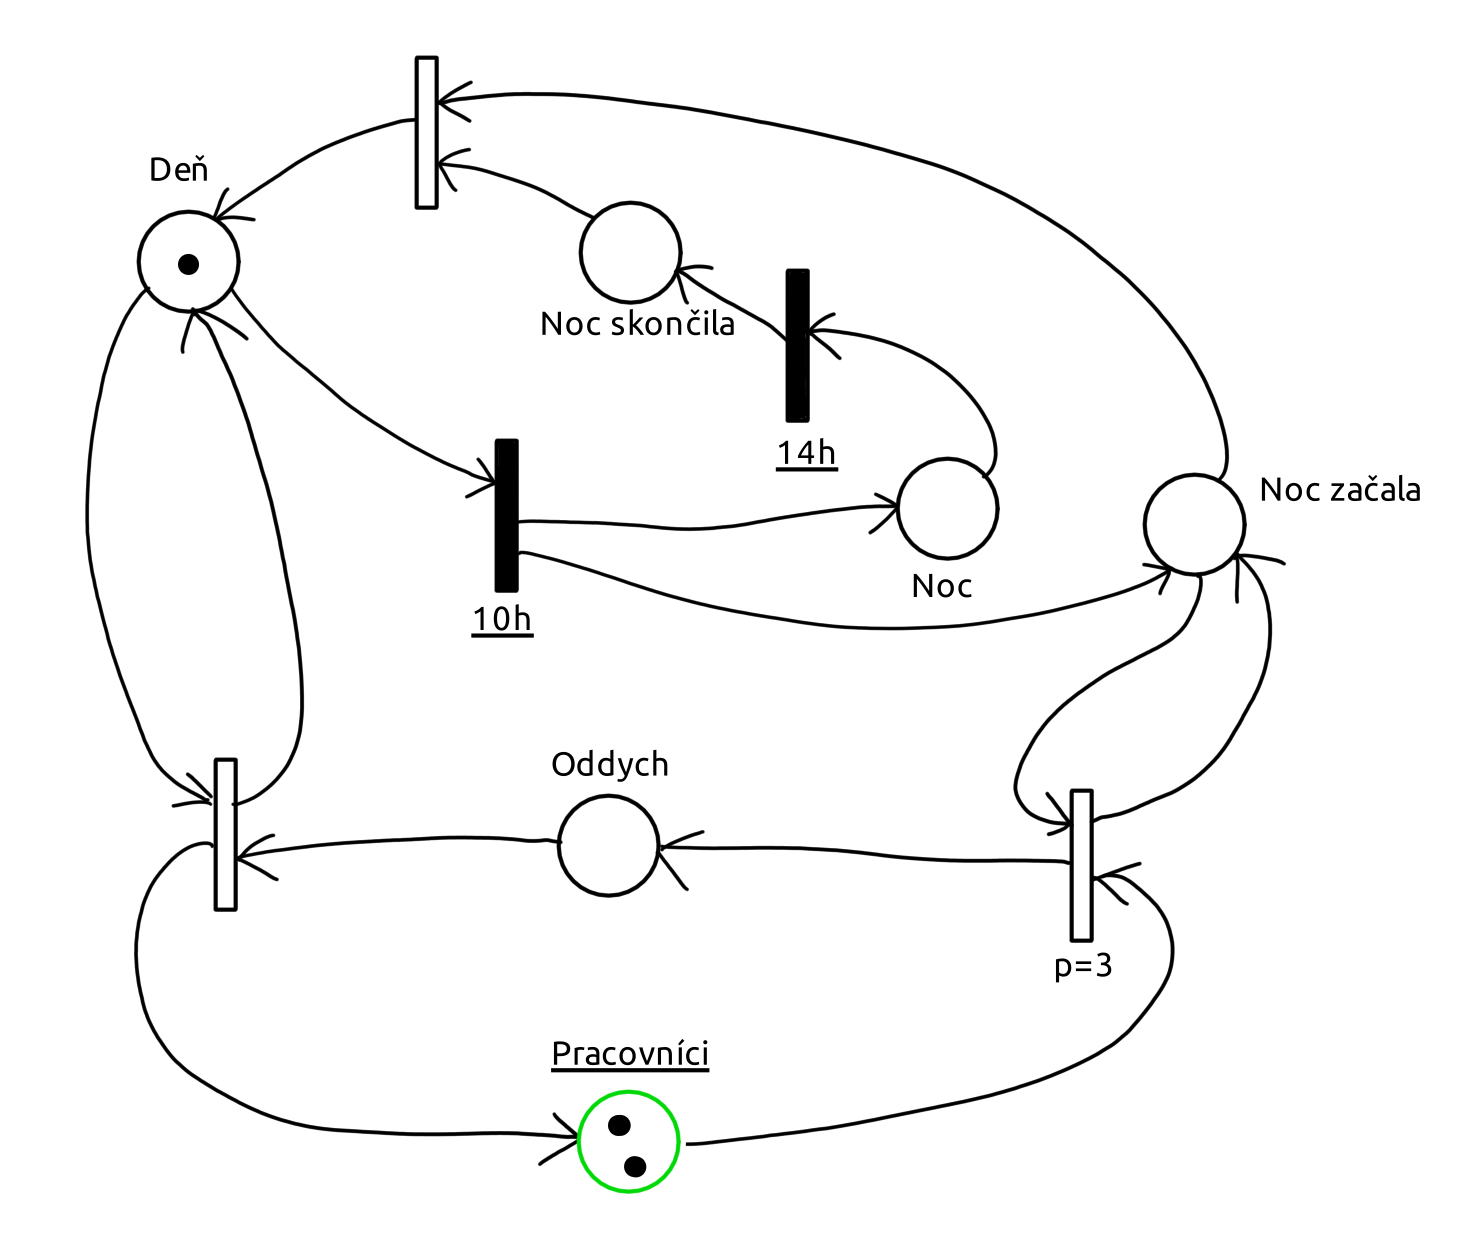
\includegraphics[scale=0.8]{ims_den-noc_cyklus.png}
    \caption{Časť zobrazujúca pracovnú dobu}
    \label{fig:petri_net_worktime}
\end{figure}
Stav, ktorý reprezentuje pracovníkov, je farebne odlíšený, pretože sa v \ref{fig:petri_net_work_process}. časti objavuje veľakrát. Takto bola sieť nakreslená, aby bola jednoduchšie pochopiteľná, keďže mať len jedno miesto na pracovníkov by bolo veľmi obtiažne nakresliť prehľadne.

Všetky hodnoty, ktoré sa môžu pri simulácii meniť pomocou vstupných parametrov sú naznačené podčiarknutím.
\begin{landscape}
\begin{figure}
    \centering
    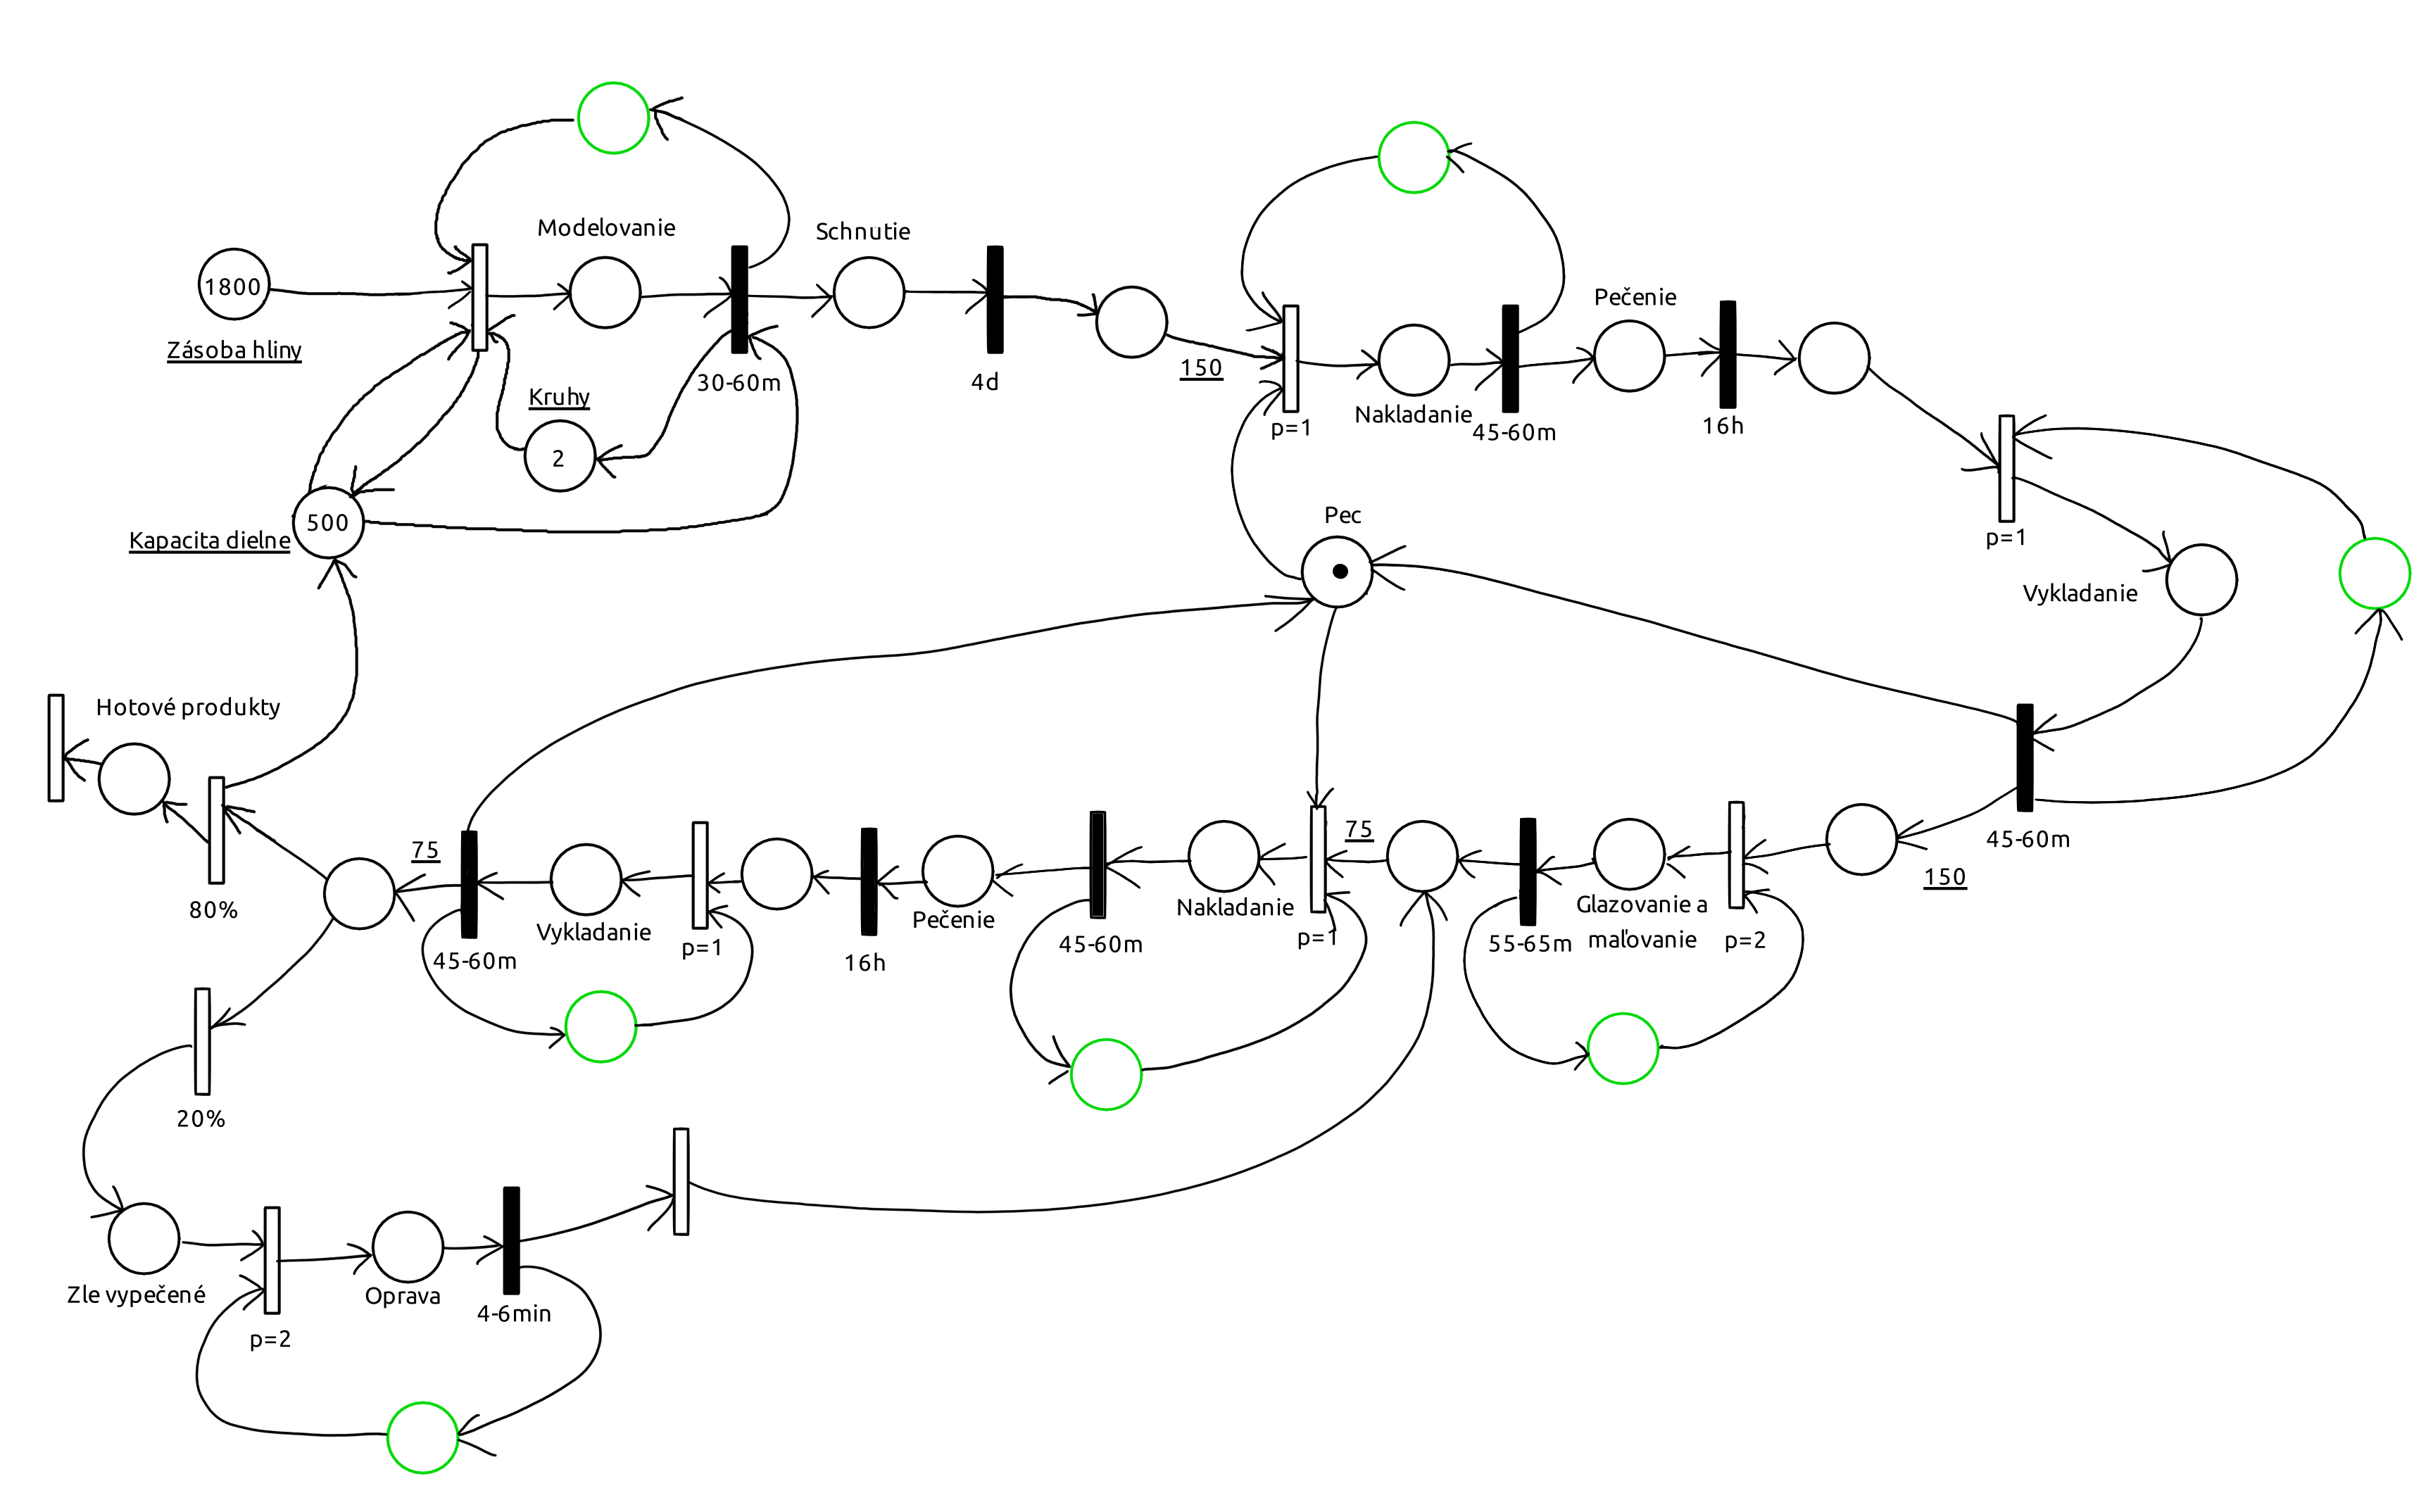
\includegraphics[scale=0.8]{ims_pracovny_cyklus.png}
    \caption{Časť zobrazujúca pracovný proces}
    \label{fig:petri_net_work_process}
\end{figure}
\end{landscape}

\end{document}
